\documentclass[rinkou,a4paper,uplatex]{ieicej}
\usepackage{graphicx}
\usepackage{url}
\usepackage{paralist}
\usepackage{nidanfloat}
\usepackage{ascmac}
\usepackage{fancybox}
\usepackage{amsmath}
\usepackage{amssymb}
\usepackage{amsfonts}
\usepackage{pifont}
\usepackage{multirow}
\usepackage{comment}

% UserSetting
\newenvironment{narrow}{\baselineskip=3mm}

\setcounter{page}{1}
\vol{98}%year
\no{12}%month
\day{14}%day

\jtitle{輪講資料テンプレ}%title
\jsubtitle
\authorlist{
 \authorentry{輪講 太郎}{Taro RINKOU}{}
} \vspace{-3mm}
\begin{document}

\maketitle

\section{はじめに}
本輪講資料テンプレートは,電子情報通信学会の和文誌テンプレートのクラスファ
イル(ieicej.cls)を改造したものです.
発表年月日は,それぞれ上部の
\begin{itemize}
 \item \textbackslash vol\{年 - 1917\}
 \item \textbackslash no\{月\}
 \item \textbackslash day\{日\}
\end{itemize}
で編集可能です.

参考文献\cite{ref}は\textbackslash cite{ラベル名}で参照できます.ラベル
名はユニークであれば自由に設定可能です.

%%%%%%%%%%%%%%%%%%%%%%%%%%%%%%%%%%%%%%%%%%%%%%%%%%%%%%%%%
\begin{figure}[hh]
\centering
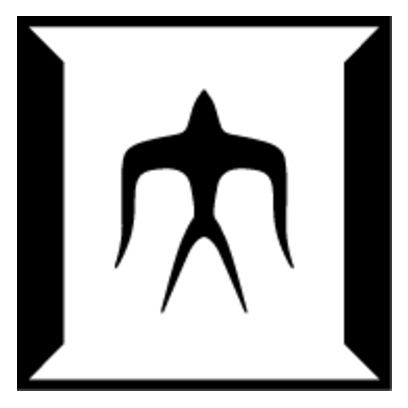
\includegraphics[scale=0.5]{fig.eps}
\caption{サンプル図}\label{tsubame}
\end{figure}
%%%%%%%%%%%%%%%%%%%%%%%%%%%%%%%%%%%%%%%%%%%%%%%%%%%%%%%%%

\begin{thebibliography}{9} % 文献数が10未満の時 {9}  文献数が10以上の時 {99}
\bibitem{ref}
 T. Rinkou, ``Hogehoge,'' IEICE Trans. Commun., vol. E00-B, no. 0,
	pp. 1-10, Feb. 2008.
\end{thebibliography}

\end{document}
